\documentclass[11pt,table,final,xcolor={usenames,dvipsnames,table},handout]{beamer}
\usetheme[]{Frankfurt}


\usepackage{listings}
\usepackage{multimedia} % Movies
\usepackage{fancyvrb,relsize}
\usepackage{commath}
\usepackage{graphicx}
\usepackage{array}
\usepackage{longtable}
\usepackage{algpseudocode} 
\usepackage{multirow}
\usepackage[math]{iwona}
\usepackage{wasysym}
% \usepackage[fleqn]{amsmath}
\usepackage{amssymb}
\usepackage{siunitx}
\usepackage{tikz} % Drawing
\usepackage{pgfplots}
\usepackage{pgfplotstable}
% \usepackage{fontspec}

% Presentation settings
\rowcolors[]{1}{maincolor!20}{maincolor!10}

\newcommand{\Fo}{\ensuremath{\mathit{Fo}}}

\lstset{language=Matlab,%
    %basicstyle=\color{red},
    basicstyle=\scriptsize\ttfamily,
    breaklines=true,%
    morekeywords={matlab2tikz},
    keywordstyle=\color{blue},%
    morekeywords=[2]{1}, keywordstyle=[2]{\color{black}},
    identifierstyle=\color{black},%
    stringstyle=\color{mylilas},
    commentstyle=\color{mygreen},%
    showstringspaces=false,%without this there will be a symbol in the places where there is a space
    numbers=none,%
%     numberstyle={\tiny \color{black}},% size of the numbers
%     numbersep=-2pt, % this defines how far the numbers are from the text
%     emph=[1]{for,end,break},emphstyle=[1]\color{red}, %some words to emphasise
emph=[2]{ones,int,str2double,long,single,simplify,diff,log,atan,solve,vpa,syms,doc,int,simplify,diff,log,atan,syms,interp3,interpn,histogram,ribbon,contourf,fzero,feval,fminsearch,fsolve,fminbnd,ezplot,varargin,optimset,odeset,ode15s,plotyy,ones,linprog,cftool,optimset,lsqnonlin}, emphstyle=[2]{\color{blue}},
    backgroundcolor=\color{gray!15},frame=tlbr, framerule=0pt,
    escapeinside={(*@}{@*)}
}

% To have the navigation circles without declaring subsections
\usepackage{remreset}% tiny package containing just the \@removefromreset command
\makeatletter
\@removefromreset{subsection}{section}
\makeatother
\setcounter{subsection}{1}

% For convenient figure inclusion
\DeclareGraphicsExtensions{.pdf,.png,.jpg}
\graphicspath{ {../img/} }


% \setmainfont{Yanone Kaffeesatz}
% \setmathfont(Digits,Latin,Greek)[Numbers={Lining,Proportional}]{Gentium Plus}

% TU/e colors
\definecolor{tuered}{RGB}{247,49,49}
\definecolor{tuefuchsia}{RGB}{214,0,74}
\definecolor{tuelila}{RGB}{214,0,123}
\definecolor{tuepurple}{RGB}{173,32,173}
\definecolor{tuedblue}{RGB}{16,16,115}
\definecolor{tueblue}{RGB}{0,102,204}
\definecolor{tuelblue}{RGB}{0,162,222}
\definecolor{tueorange}{RGB}{255,154,0}
\definecolor{tueyellow}{RGB}{255,221,0}
\definecolor{tuedyellow}{RGB}{206,223,0}
\definecolor{tuegreen}{RGB}{132,210,0}
\definecolor{tuedgreen}{RGB}{0,172,130}
\definecolor{tueblue2}{RGB}{0,146,181}

% For Matlab script colors
\definecolor{mygreen}{RGB}{28,172,0} % color values Red, Green, Blue
\definecolor{mylilas}{RGB}{170,55,241}

\makeatletter
% \definecolor{beamer@blendedblue}{rgb}{0.5,0.5,0.3} % changed this
\useoutertheme{smoothbars}
\useinnertheme{circles}

%%%%%%%%%%%%%%%%%%%%%%%%%%%%%%%%%%%%%%%%%%%%%%%%%%%%%%%%%%%%%%%%%%%%%%%%%%%
\definecolor{maincolor}{named}{tuelblue}
\definecolor{textcolorfg}{named}{white}
\definecolor{tuealert}{named}{tueblue}
%%%%%%%%%%%%%%%%%%%%%%%%%%%%%%%%%%%%%%%%%%%%%%%%%%%%%%%%%%%%%%%%%%%%%%%%%%%

\setbeamercolor{normal text}{fg=black,bg=white}
\setbeamercolor{alerted text}{fg=tuealert}
\setbeamercolor{example text}{fg=tuegreen!50!black}

\setbeamercolor{background canvas}{parent=normal text,bg=white}
\setbeamercolor{background}{parent=background canvas}

\setbeamercolor{title}{bg=maincolor,fg=textcolorfg} % Presentation title colors
\setbeamercolor{structure}{fg=maincolor,bg=textcolorfg}
\setbeamercolor{section in head/foot}{fg=textcolorfg,bg=maincolor}
\setbeamercolor{palette primary}{fg=textcolorfg,bg=maincolor} % changed this

\setbeamercolor{palette primary}{fg=maincolor,bg=textcolorfg} % changed this
\setbeamercolor{palette secondary}{use=structure,fg=structure.fg!100!tueblue} % changed this
\setbeamercolor{palette tertiary}{use=structure,fg=structure.fg!100!tuered} % changed this

\setbeamertemplate{navigation symbols}{} % ( Dont use )
\setbeamercolor{navigation symbols}{use=structure,fg=structure.fg!40!bg}
\setbeamercolor{navigation symbols dimmed}{use=structure,fg=structure.fg!20!bg}

\setbeamercolor{block title}{fg=textcolorfg,bg=maincolor}
\setbeamercolor{block body}{fg=black,bg=maincolor!10}

\def\colorize<#1>{%
  \temporal<#1>{\color{tuedblue!40!gray!40}}{\color{tuealert}}{\color{black}}}
  
\setlength{\mathindent}{0pt}

\makeatother

% Colored urls
\hypersetup{colorlinks,linkcolor=,urlcolor=tueblue}

% Vector format
\renewcommand{\vec}[1]{\mathbf{#1}}

\usetikzlibrary{decorations} % Drawing
\usetikzlibrary{patterns}
\usetikzlibrary{positioning}
\usetikzlibrary{shadows}
\usetikzlibrary{calc}
\usetikzlibrary{arrows}
\usetikzlibrary{decorations}
\usetikzlibrary{plotmarks}
\usetikzlibrary{shapes}
\usetikzlibrary{shadings}
\usetikzlibrary{intersections}
% Blocks
\tikzset{block/.style={rectangle,draw=maincolor,fill=maincolor!20,text width=10em,text centered,rounded corners,minimum height=4em,thick}}
\tikzset{emphblock/.style={rectangle,draw=maincolor,text centered,rounded corners,thick,top color=maincolor!10,bottom color=maincolor!30}}
% Dots
\tikzset{dot/.style={draw=tuered,circle,thick,minimum size=1mm,inner sep=0pt,outer sep=0pt,fill=white}}
\tikzset{fdot/.style={circle,draw=black,fill=black,,inner sep=1.5pt}}
\tikzset{gdot/.style={circle,draw=black,inner sep=3pt}}
\tikzset{cross/.style={cross out, draw=black, fill=none, minimum size=2*(#1-\pgflinewidth), inner sep=0pt, outer sep=0pt}, cross/.default={4pt}}
% Graphs and lines
\tikzset{line/.style={black,>=stealth',semithick}}
\tikzset{graph/.style={smooth,samples=400,tuered,semithick}}
\tikzset{interp/.style={dot,draw=tuealert,inner sep=1.5pt,minimum size=4pt,color=tuealert,fill=none}}
\tikzset{intblock/.style={line,draw=tuefuchsia,fill=tuefuchsia!50!white,fill opacity=0.3,opacity=0.6}}
\tikzset{intdot/.style={line,dot,draw=tuefuchsia,fill=tuefuchsia,opacity=0.6}}
\tikzset{gridline/.style={lightgray,ultra thin,dashed}}


\newcolumntype{L}[1]{>{\raggedright\arraybackslash}p{#1}}
\newcolumntype{R}[1]{>{\raggedleft\arraybackslash}p{#1}}

% \pgfplotsset{
% % every axis y label/.append style={at={axis cs:14,14},rotate=0,anchor=south east}
% exery axis/.style={ylabel near ticks},
% }


\renewcommand*\familydefault{\sfdefault}  % Use sans font

% \usepackage{pgfpages}
% \pgfpagesuselayout{4 on 1}[border shrink=5mm]

\usepackage[customcolors]{hf-tikz}

\title{Linear equation solvers}
\subtitle{Iterative methods}

\author[I.~Roghair]{\underline{Ivo~Roghair}, Martin van Sint Annaland}

\institute[SPI]{{Chemical Process Intensification,\\
  Eindhoven University of Technology}}

\date


% BEGIN PRESENTATION
\begin{document}
\lstset{language=Matlab,%
    %basicstyle=\color{red},
    basicstyle=\footnotesize\ttfamily,
    breaklines=true,%
    morekeywords={matlab2tikz},
    keywordstyle=\color{blue},%
    morekeywords=[2]{1}, keywordstyle=[2]{\color{black}},
    identifierstyle=\color{black},%
    stringstyle=\color{mylilas},
    commentstyle=\color{mygreen},%
    showstringspaces=false,%without this there will be a symbol in the places where there is a space
    numbers=none,%
%     numberstyle={\tiny \color{black}},% size of the numbers
%     numbersep=-2pt, % this defines how far the numbers are from the text
%     emph=[1]{for,end,break},emphstyle=[1]\color{red}, %some words to emphasise
    emph=[2]{ones,int,simplify,diff,log,atan,syms,doc,int,simplify,diff,log,atan,syms,interp3,interpn,histogram,ribbon,contourf,fzero,feval,fminsearch,fsolve,fminbnd,ezplot,varargin,optimset,odeset,plotyy,ones,linprog,cftool,optimset,lsqnonlin}, emphstyle=[2]{\color{blue}},
    backgroundcolor=\color{gray!15},frame=tlbr, framerule=0pt,
    escapeinside={(*@}{@*)}
}

\frame[plain]{
  \titlepage
}
% \part{Solving systems of linear equations}
% \frame{\partpage}
\section{Introduction}
\subsection*{General}
\begin{frame}[label=contents]
  \frametitle{Today's outline}
  \mode<beamer>{
    \only<1>{\tableofcontents}
  }
  \only<2>{\tableofcontents[currentsection,currentsubsection]}
\end{frame}

\section{Sparse matrices}
\subsection*{Sparse matrices}

\begin{frame}[fragile]
  \frametitle{Sparse matrices}
  \begin{itemize}
    \item In many engineering cases, we deal with sparse matrices (as opposed to dense matrices)
    \item A matrix is sparse when it mostly consists of zeros
    \item Linear systems where equations depend on a limited number of variables (e.g. spatial discretization)
    \item Storing zeros is not very efficient:
    \begin{lstlisting}
>> A = eye(10000);
>> whos A
>> S = sparse(A);
>> whos S
    \end{lstlisting}
    \item Can you think of a way to achieve this?
    \item Sparse matrix formats: Yale, CRS, CCS
\end{itemize}
\end{frame}

\begin{frame}[fragile]
  \frametitle{Sparse matrix storage format}
  \begin{columns}
  \column{0.6\textwidth}
  \begin{itemize}
    \item Example: Yale storage format, storing 3 vectors:
    \begin{itemize}
      \item \lstinline$A = [5 8 3 6]$
      \item \lstinline$IA = [0 0 2 3 4]$
      \item \lstinline$JA = [0 1 2 1]$
    \end{itemize}
  \end{itemize}
  \column{0.4\textwidth}
  \[
   A = 
   \begin{bmatrix}
    0 & 0 & 0 & 0\\
    5 & 8 & 0 & 0\\
    0 & 0 & 3 & 0\\
    0 & 6 & 0 & 0
    \end{bmatrix}
  \]
  \end{columns}
  \begin{itemize}
    \item \lstinline$A$ stores the non-zero values
    \item \lstinline$IA$ stores the index in A of the first non-zero in row i
    \item \lstinline$JA$ stores the column index
    \item Note: zero-based indices are used here!
\end{itemize}
\end{frame}

\begin{frame}[fragile]
  \frametitle{Sparse matrix layout examples}
  \begin{center}
   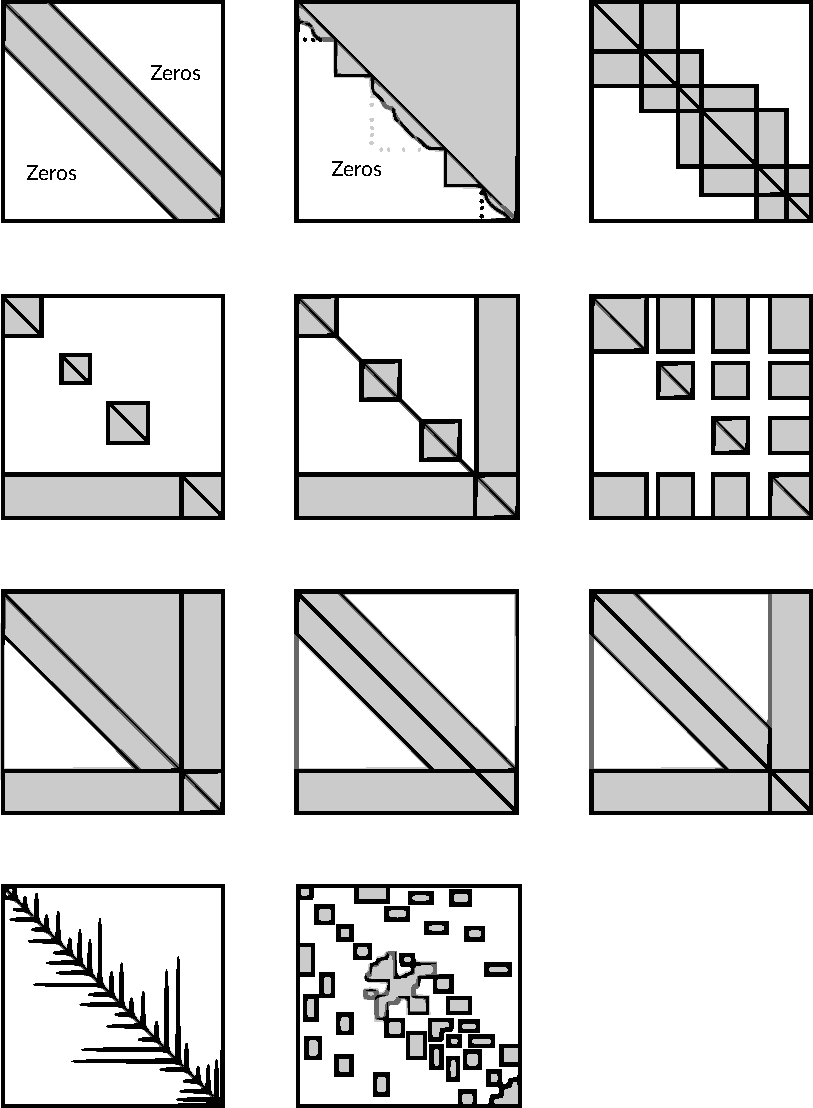
\includegraphics[height=0.8\textheight]{img/sparse-overview}
  \end{center}
\end{frame}

\section{Laplace's equation}
\subsection*{Laplace's equation}
\againframe<2>{contents}
\begin{frame}[fragile]
  \frametitle{Laplace's equation}
  \begin{columns}
  \column{0.7\textwidth}
  \begin{align*}
    \frac{\partial T}{\partial t} &= \alpha \nabla^2 T \\
    T &= \text{Temperature} \\
    \alpha &= \text{Thermal diffusivity}
  \end{align*}
  \pause
  \begin{center}
      \begin{tikzpicture}[scale=0.5]
      \draw[black,thick,->] (-0.3,-0.3)-- node[at end,anchor=north]{$x$}(7,-0.3);
      \draw[black,thick,->] (-0.3,-0.3)-- node[at end,anchor=east]{$y$} (-0.3,7);
      \draw[thick,draw=tuelblue,fill=tuegreen] (0,0) rectangle +(6,6);
      \node[anchor=west] at (6,3) {$T=T_{b4}$};
      \node[above,anchor=south] at (3,6.5) {$T=T_{b2}$};
      \node[below,anchor=north] at (3,-0.5  ) {$T=T_{b1}$};
      \node[left of=3pt] at (0,3) {$T=T_{b3}$};
%       \node at (0.3,0.3) (A) {};
%       \node at (0.3,5.7) (B) {};
%       \node at (5.7,5.7) (C) {};
%       \node at (5.7,0.3) (D) {};
%       \draw[thick,tuered] (A) -- node[midway,anchor=east] {$T=T_{b3}$} (B);
%       \draw[thick,tuegreen] (B) -- node[midway,anchor=south] {$T=T_{b2}$} (C);
%       \draw[thick,tueorange] (C) -- node[midway,anchor=east] {$T=T_{b4}$} (D);
%       \draw[thick,tuepurple] (D) -- node[midway,anchor=south] {$T=T_{b1}$} (A);
      \end{tikzpicture}
    \end{center}
    \pause
  \column{0.3\textwidth}
  In steady state:
  \[
   \nabla^2 T = 0
  \]
  \vskip2em
  \[
   \frac{\partial^2T}{\partial x^2} + \frac{\partial^2T}{\partial y^2} = 0
  \]
\end{columns}
\end{frame}

\begin{frame}[fragile]
  \frametitle{Laplace's equation}
  \begin{columns}
  \column{0.6\textwidth}
%     \vskip-2em
    \hspace*{-2em}
    \begin{tikzpicture}[scale=0.75,font=\sffamily\scriptsize]
      \foreach \x in {0,...,5}
        \foreach \y in {0,...,5} 
          {
    %        \pgfmathtruncatemacro{\label}{\x - 5 *  \y +21}
          \ifthenelse{\x=0 \OR \x=5 \OR \y=0 \OR \y=5}{\node [gdot,fill=tuered]  (\x\y) at (1.5*\x,1.5*\y) {};}
          \node [gdot,fill=tueblue]  (\x\y) at (1.5*\x,1.5*\y) {};} 

        \foreach \x [count=\xi] in {0,...,4}
          \foreach \y [count=\yi] in {0,...,4}  
            \draw (\x\y)--(\x\yi)-- (\xi\yi)--(\xi\y)--(\x\y);% (\y\x)--(\yi\x) ;
        
        \onslide<2->{
	  \node[anchor=east] at (00.west) {$j=1$};
	  \node[anchor=east] at (01.west) {$j=2$};
	  \node[anchor=east] at (02.west) {$j=3$};
	  \node[anchor=east] at (04.west) {$j=N_y-1$};
	  \node[anchor=east] at (05.west) {$j=N_y$};
	  \node[anchor=north] at (00.south) {$i=1$};
	  \node[anchor=north] at (10.south) {$i=2$};
	  \node[anchor=north] at (20.south) {$i=3$};
	  \node[anchor=north] at (40.south) {$i=N_x-1$};
	  \node[anchor=north west] at (50.south) {$i=N_x$};
	}
	
	\onslide<3->{
	  \node[anchor=south west] at (00.north east) {$T_1$};
	  \node[anchor=south west] at (10.north east) {$T_2$};
	  \node[anchor=south west] at (20.north east) {$T_3$};
	  \node[anchor=south west] at (30.north east) {$T_4$};
	  \node[anchor=south west] at (40.north east) {$T_5$};
	  \node[anchor=south west] at (50.north east) {$T_6$};
	  \node[anchor=south west] at (01.north east) {$T_{N_x+1}$};
	  \node[anchor=south west] at (11.north east) {$T_{N_x+2}$};
	  \node[anchor=south west] at (21.north east) {$T_{N_x+3}$};
	  \node[anchor=south west] at (51.north east) {$T_{2N_x}$};
	  \node[anchor=south]      at (55.north) {$T_{(N_y-1)N_x+1}$};
	}
      \end{tikzpicture}
%     \end{center}
  \hfill
  \column{0.35\textwidth}
  \begin{itemize}
    \item<1-> Define a grid of points in $x$ and $y$
    \item<2-> Index of the grid points using 2D coordinates $i$ and $j$
    \item<3> Set up the equations using a 1D index system: $T_{i,j}=T_{i+N_x(j-1)}$
  \end{itemize}
  \end{columns}
\end{frame}

\begin{frame}[fragile]
  \frametitle{Laplace's equation}
  Estimate the second-order differentials: assume a piece-wise linear profile in the temperature: \vskip1em
  \begin{columns}
  \column{0.5\textwidth}
    \begin{tikzpicture}[scale=0.7,node distance=5mm]
      \draw[black,thick,->] (0,0)-- node[at end,anchor=north]{$x$}(7,0);
      \draw[black,thick,->] (0,0)-- node[at end,anchor=east ]{$T$}(0,5);
      \node [gdot,fill=tuered] (n1) at (1,0) {};
      \node [gdot,fill=tuered] (n2) at (3,0) {};
      \node [gdot,fill=tuered] (n3) at (5,0) {};
      \node [anchor=south,dot,color=black,fill=black] (e1) at (1,1) {};
      \node [anchor=south,dot,color=black,fill=black] (e2) at (3,2) {};
      \node [anchor=south,dot,color=black,fill=black] (e3) at (5,4) {};
      \node [below=1mm of e1.center,anchor=north west] (e4) {$T_{i-1}$};
      \node [below=1mm of e2.center, anchor=north west] (e5) {$T_{i}$};
      \node [below=1mm of e3.center,anchor=north west] (e6) {$T_{i+1}$};
      \draw[black,thick] (e1.center) -- (e2.center) -- (e3.center);
      \draw[black,thick,<->] (1,-0.5) -- node[midway, below] {$\Delta x$} (2.9,-0.5);
      \draw[black,thick,<->] (3.1,-0.5) -- node[midway, below] {$\Delta x$} (5,-0.5);
      \end{tikzpicture}
%     \end{center}
  \hfill
  \column{0.35\textwidth}
  \begin{align*}
    \frac{\partial^2T}{\partial x^2} \approx \frac{\left.\frac{\partial T}{\partial x}\right|_{i+\frac{1}{2}}-\left.\frac{\partial T}{\partial x}\right|_{i-\frac{1}{2}}}{\Delta x} \\[15pt]
    \approx \frac{ \frac{\left(T_{i+1,j}-T_{i,j}\right)}{\Delta x} - \frac{\left(T_{i,j}-T_{i-1,j}\right)}{\Delta x}}{\Delta x}\\[15pt]
    = \frac{T_{i+1,j}-2T_{i,j}+T_{i-1,j}}{(\Delta x)^2}
  \end{align*}
  \end{columns}
\end{frame}

\begin{frame}[fragile]
  \frametitle{Laplace's equation}
  The $y$-direction is derived analogously, so that the 2D Laplace's equation is discretized as:
  \[
    \frac{T_{i+1,j}-2T_{i,j}+T_{i-1,j}}{(\Delta x)^2} + \frac{T_{i,j+1}-2T_{i,j}+T_{i,j-1}}{(\Delta y)^2} = 0
  \]
  \pause
  Use a single index counter ${k=i+N_x(j-1)}$, so that the equation becomes:
  \[
    \frac{T_{k+1}-2T_k+T_{k-1}}{(\Delta x)^2} + \frac{T_{k+N_x}-2T_k+T_{k-N_x}}{(\Delta y)^2} = 0
  \]
  \pause
  For an equal spaced grid $\Delta x = \Delta y = 1$:
  \tikz{\node[emphblock, text width=\textwidth,]{\[
   T_{k-N_x} + T_{k-1} - 4T_k + T_{k+1} + T_{k+N_x} = 0
   \]
   \[
      \Rightarrow AT=b
   \]\vskip1ex
   %\Rightarrow T_k = \frac{T_{k-N_x} + T_{k-1} + T_{k+1} + T_{k+N_x}}{4}
  };}
\end{frame}

\section{Creating a sparse system}
\subsection*{A sparse matrix}
\againframe<2>{contents}
\begin{frame}[fragile]
  \frametitle{Creating the linear system}
  \vskip-1em
  \[
   T_{k-N_x} + T_{k-1} - 4T_k + T_{k+1} + T_{k+N_x} = 0
  \]
  Create a \emph{banded} matrix $A$: the main diagonal $k$ contains -4, whereas the bands at $k-1$, $k+1$, $k-N_x$ and $k+N_x$ contain a 1. Boundary cells just contain a 1 on the main diagonal so that the temperature is equal to $T_b$ (e.g. $T_1 = 1T_b$).\\
  \vskip1em
  \hspace*{-2em}
  ${
    \begin{bmatrix}
      1 & 0 & 0 & 0 & 0 & 0 & 0 & 0 & \cdots & 0\\
      0 & 1 & 0 & 0 & 0 & 0 & 0 & 0 & \cdots & 0\\
    \vdots & \vdots & \vdots & \vdots & \vdots & \vdots & \vdots & \vdots & \ddots & \vdots\\
     \cdots & 1 & \cdots & 1 & -4 & 1 &\cdots & 1 & \ddots & 0\\
     0 & \cdots & 1 & \cdots & 1 & -4 & 1 &\cdots & 1 & \vdots\\
     \vdots & \vdots & \vdots & \vdots & \vdots & \vdots & \vdots & \vdots & \ddots & \vdots\\
     0 & 0 & 0 & 0 & 0 & 0 & 0 & 0 & 1 & 0\\
     0 & 0 & 0 & 0 & 0 & 0 & 0 & 0 & 0 & 1\\
    \end{bmatrix}
    \begin{bmatrix}
    T_1\\
    T_2\\
    \vdots\\
    T_k\\
    T_k+1\\
    \vdots\\
    T_{(N_y-1)N_x}\\
    T_{(N_y-1)N_x+1}
   \end{bmatrix} = 
   \begin{bmatrix}
    T_b\\
    T_b\\
    \vdots\\
    0\\
    0\\
    \vdots\\
    T_b\\
    T_b
   \end{bmatrix}}$
\end{frame}

\begin{frame}[fragile]
  \frametitle{Creating the linear system}
  \vskip-1em
  \[
   T_{k-N_x} + T_{k-1} - 4T_k + T_{k+1} + T_{k+N_x} = 0
  \]
  Create a \emph{banded} matrix $A$ in Matlab, by setting the coefficients for the internal cells:
  \begin{lstlisting}
% Grid size
Nx=5;  %number of points along x direction
Ny=5;  %number of points in the y direction
Nc=Nx*Ny; % Total number of points

e = ones(Nc,1);
A = spdiags([e,e,-4*e,e,e],[-Nx,-1,0,1,Nx],Nc,Nc);
  \end{lstlisting}
  The function \lstinline$spdiags$ uses the following arguments:
  \begin{itemize}
   \item The coefficients that have to be put on the diagonals arranged as columns in a matrix
   \item The position of the bands with respect to the main diagonal
   \item Size of the resulting matrix (in our case square $N_xN_y \times N_xN_y$)
  \end{itemize}
\end{frame}

\begin{frame}[fragile]
  \frametitle{Matrix sparsity}
  \begin{columns}
  \column{0.5\textwidth}
  
  \begin{itemize}
   \item Let's check the matrix layout:
   \begin{lstlisting}
>> spy(A)
   \end{lstlisting}
    \item This command shows the non-zero values of a matrix
    \item Apart from the main diagonal, there are offset bands!
  \end{itemize}
  \column{0.5\textwidth}
    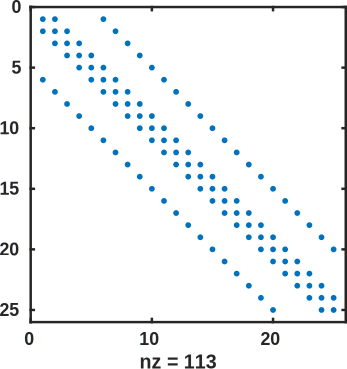
\includegraphics[width=\columnwidth]{img/sparse_matlab}
  \end{columns}
\end{frame}

\begin{frame}[fragile]
  \frametitle{LU decomposition of a sparse matrix}
  \begin{columns}
  \column{0.35\textwidth}
   \begin{lstlisting}
>> [L,U,P] = lu(A)
>> subplot(1,2,1)
>> spy(L)
>> subplot(1,2,2)
>> spy(U)
   \end{lstlisting}
  \column{0.65\textwidth}
  \pause
  \begin{itemize}
   \item With LU decomposition we produce matrices that are less sparse than the original matrix.
   \item Sparse storage often required, and also numerical techniques that fully utilizes this!
  \end{itemize}\vskip2em
  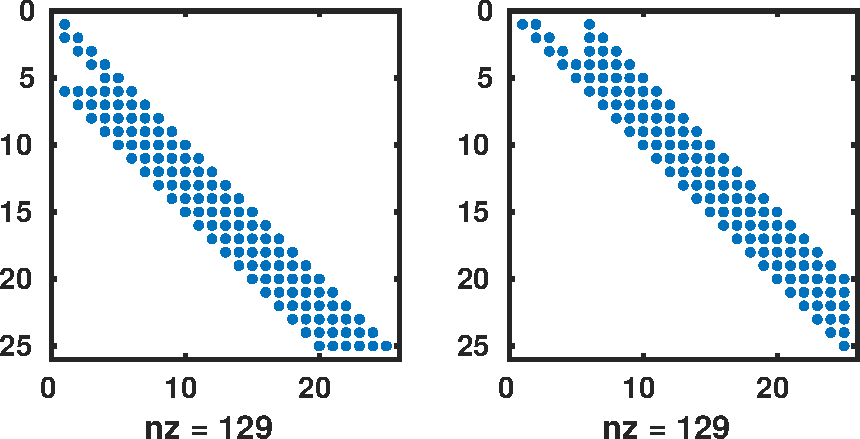
\includegraphics[width=\columnwidth]{img/sparse_lu}
  \end{columns}
\end{frame}

\subsection*{Boundary conditions}
\begin{frame}[fragile]
  \frametitle{About boundary conditions}
  \begin{itemize}
   \item For the nodes on the boundary, we have a simple equation:
    \[
      T_{k,\text{boundary}} = \text{Some fixed value}
    \]
    \item However, we have set all nodes to be a function of their neighbors...
    \item Find the boundary node indices using $k = i + Nx(j-1)$
    \begin{itemize}
      \item \lstinline$i = 1$, \lstinline$j = 1:Ny$
      \item \lstinline$i = Nx$, \lstinline$j = 1:Ny$
      \item \lstinline$j = 1$, \lstinline$i = 1:Nx$
      \item \lstinline$j = Ny$, \lstinline$i = 1:Nx$
    \end{itemize}
    \item Reset the row in $A$ to zeros, set $A_{kk}$ = 1
    \item Set value in rhs: $b_k = T_{k,\text{boundary}}$
    \item Boundary conditions are often more elaborate to implement! See \lstinline$setBoundaryConditions.m$.
  \end{itemize}
\end{frame}

\subsection*{Solving the equation}
\begin{frame}[fragile]
  \frametitle{A full program, including solver}
  The program and auxiliary functions are on Canvas (\lstinline$solveLaplaceEq.m$)
\begin{lstlisting}[linewidth=1.05\textwidth]
function [x,y,T,A] = solveLaplaceEq(Nx,Ny)
% Solves the steady-state Laplace equation 

Tb = [10 20 30 40]; % Fixed boundary temperatures

% Fill sparse matrix with [1 1 -4 1 1]
e = ones(Nx*Ny,1);
A = spdiags([e,e,-4*e,e,e],[-Nx,-1,0,1,Nx],Nx*Ny,Nx*Ny);
b = zeros(Nx*Ny,1);

[A,b] = setBoundaryConditions(A,b,Tb,Nx,Ny);

T = A\b;  % Solve matrix
Tc = reshape(T,[Nx,Ny]); % Reshape x-vec to mat Nx,Ny
[xc yc] = meshgrid(1:Nx,1:Ny); % Get position arrays
surf(xc,yc,Tc); % Surface plot
\end{lstlisting}
\end{frame}

\begin{frame}[fragile]
  \frametitle{Sample results}
  Solved for a $20\times20$ system with $T_b=\left[10\ 20\ 30\ 40\right]$.\vskip1em
  \begin{center}
    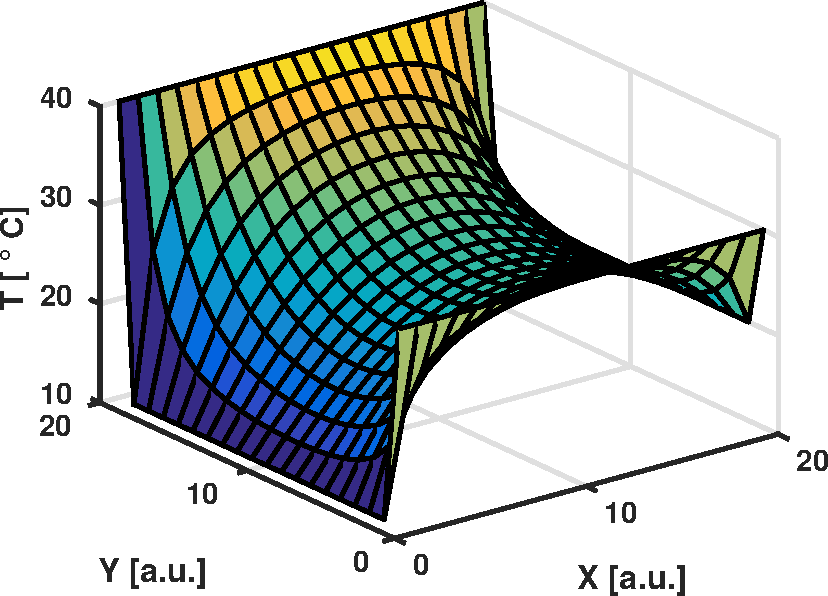
\includegraphics[width=0.8\textwidth]{img/laplace_20x20}
  \end{center}
\end{frame}

\begin{frame}[fragile]
  \frametitle{LU decomposition}
  \begin{itemize}
    \item LU decomposition and Gaussian elimination on a matrix like $A$ requires more memory (with 3D problems, the offset in the diagonal would even be bigger!)
    \item In general extra memory allocation will not be a problem for MATLAB
    \item MATLAB is clever, in that sense that it attempts to reorder equations, to move elements closer to the diagonal)
  \end{itemize} \pause
  Alternatives for Gaussian elimination
  \begin{itemize}
    \item Use iterative methods when systems are large and sparse.
    \item Often such systems are encountered when we want to solve PDE’s of higher dimensions
  \end{itemize}
\end{frame}

\section{Iterative methods}
\subsection*{Introduction}
\againframe<2>{contents}

\begin{frame}[fragile]
  \frametitle{Examples of iterative methods}
  \begin{itemize}
    \item Jacobi method
    \item Gauss-Seidel method
    \item Succesive over relaxation \vskip2em
    \item \lstinline$bicg$ --- Bi-conjugate gradient method
    \item \lstinline$pcg$ --- preconditioned conjugate gradient method
    \item \lstinline$gmres$ --- generalized minimum residuals method
    \item \lstinline$bicgstab$ --- Bi-conjugate gradient method
  \end{itemize}
\end{frame}

\subsection*{Jacobi method}
\begin{frame}[fragile]
  \frametitle{The Jacobi method}
  \begin{itemize}
     \item In our example we derived the following equation:
    \[
     T_{k-N_x} + T_{k-1} - 4T_k + T_{k+1} + T_{k+N_x} = 0
    \]
    \item Rearranging gives:
    \[
      T_k = \frac{T_{k-N_x} + T_{k-1} + T_{k+1} + T_{k+N_x}}{4}
    \]\pause
    \item In the Jacobi scheme the iteration proceeds as follows:
    \begin{enumerate}
      \item Start with an initial guess for the values of $T$ at each node\pause
      \item Compute updated values and store a new vector:
        \[
          T_k^\text{new} = \frac{T_{k-N_x}^\text{old} + T_{k-1}^\text{old} + T_{k+1}^\text{old} + T_{k+N_x}^\text{old}}{4}
        \]\pause
      \item Do this for all nodes\pause
      \item Repeat the procedure until converged
    \end{enumerate}
  \end{itemize}
\end{frame}

\begin{frame}[fragile]
  \frametitle{Jacobi method for Laplace's equation}
  \vskip-1em
  See \lstinline$laplace_jacobi.m$ (from Canvas)
  \begin{lstlisting}[basicstyle=\scriptsize\ttfamily]
% Grid size
nx = 40; ny = 40; (*@ \pause @*)
% The temperature field + boundaries at old and new times
T = zeros(nx,ny);
T(1,:) = 40;  % Left 
T(nx,:) = 60; % Right
T(:,1) = 20;  % Bottom
T(:,ny) = 30; % Top (*@ \pause @*)
Tnew = T; (*@ \pause @*)
% For plotting
[x y] = meshgrid(1:nx, 1:ny); (*@ \pause @*)
for iter = 1:1000 
  for i = 2:nx-1
    for j = 2:ny-1 
      Tnew(i,j) = (T(i-1,j)+T(i+1,j)+T(i,j-1)+T(i,j+1))/4.0;
    end
  end (*@ \pause @*)
  surf(x,y,Tnew);
  title(['Iteration: ' num2str(iter)]);
  drawnow
  T = Tnew; % Update T
end
  \end{lstlisting}
\end{frame}

\begin{frame}[fragile]
  \frametitle{About the straightforward implementation}
  \begin{itemize}
  
   \item The method as implemented works fine for a simple Laplace equation
%    \item We did not take into account the thermal diffusivity (set to unity)
%    \item We did not take into account the grid spacing (set to unity)
   \item For generic systems of linear equations, the implementation cannot be used.
  \end{itemize}\vskip2em\pause
 \tikz{\node[emphblock,text width=\textwidth]{We will now introduce the Jacobi method so it can be used for generic systems of linear equations.};}
\end{frame}

\begin{frame}[fragile]
  \frametitle{The Jacobi method with matrices}
  We can split our (banded) matrix $A$ into a diagonal matrix $D$ and a remainder $R$:\vskip1em
  \[
   A \quad =\quad  D \quad + \quad R
  \]
 \vskip2em
  \scalebox{0.6}{
  $
   \begin{bmatrix}
    \times & \times &  &  &  &  & \times &  & \\
    \times & \times & \times &   &   &   &   & \times &    \\
           & \times & \times & \times &   &   &   &   & \times \\
           &   & \times & \times & \times &   &   &   &   \\
      &   &   & \times & \times & \times &   &   &    \\
      &   &   &   & \times & \times & \times &   &   \\
      \times &   & &   &   & \times & \times & \times &   \\
      &   \times &   & &   &   & \times & \times & \times \\
      &   &   \times &   & &   &   & \times & \times \\
   \end{bmatrix} = 
   \begin{bmatrix}
    \times &  &  &  &  &  &  &  & \\
     & \times &  &   &   &   &   &  &    \\
           &  & \times &  &   &   &   &   &  \\
           &   &  & \times &  &   &   &   &   \\
     &   &   &  & \times &  &   &   &    \\
      &  &   &   &  & \times &  &   &   \\
      &   &  &   &   &  & \times &  &   \\
      &   &   &  &   &   &  & \times &  \\
      &   &   &   &  &   &   &  & \times \\
   \end{bmatrix} + 
   \begin{bmatrix}
     & \times &  &  &  &  & \times &  & \\
    \times &  & \times &   &   &   &   & \times &    \\
           & \times &  & \times &   &   &   &   & \times \\
           &   & \times &  & \times &   &   &   &   \\
      &   &   & \times &  & \times &   &   &    \\
      &   &   &   & \times &  & \times &   &   \\
      \times &   & &   &   & \times &  & \times &   \\
      &   \times &   & &   &   & \times &  & \times \\
      &   &   \times &   & &   &   & \times &  \\
   \end{bmatrix}$}
\end{frame}

\begin{frame}[fragile]
  \frametitle{Jacobi method: solving a system}
  \begin{itemize}
   \item Now we can solve AT=b by:
   \begin{align*}
   AT&=b\\
     (D+R)T &= b \\
      DT &= b -RT \\
      DT^\text{new} &= b - RT^\text{old} \\
       T^\text{new} &= D^{-1}(b-RT^\text{old})
   \end{align*}
   \item Using the $n$ and $n+1$ notation for old and new time steps, we find in general:
   \[
    x^{n+1} = D^{-1}\left(  b-Rx^n\right)
   \]
   \[
    x_i^{n+1} = \frac{1}{A_{ii}}\left(b_i - \sum_{j\neq i} A_{ij}x_j^n\right)
   \]
  \end{itemize}
\end{frame}

\begin{frame}[fragile]
  \frametitle{Diagram of the Jacobi method}
  \begin{tikzpicture}[scale=0.5,font=\tiny,node distance = 25pt, auto,->=stealth,point/.style={circle,fill=red,minimum size=0pt,inner sep=0pt}]
    \tikzstyle{block2} = [rectangle,minimum height=1em,draw=maincolor,fill=maincolor!20,text centered,rounded corners,minimum height=2em,thick,text width=1.5cm]
    \node[block2]                 (start) {Set $T^\text{old}$ = a guess};
    \node[block2, right=of start,visible on=<2->] (calc)  {Calculate the new node solution with previous values.};
    \node[block2, right=of calc,visible on=<3->] (check1) {Have all nodes been updated?};
    \node[block2, right=of check1,,visible on=<5->] (tol) {Tolerance check: $\left(Ax-b \leq \text{tol}\right) $?};
    \node[block2, above=of check1,visible on=<4->] (next) {Move to next node};
    \node[block2, above=of tol,visible on=<6->] (update) {Update $T^\text{old}=T^\text{new}$};
    \node[block2, below=of tol,visible on=<8->] (answer) {Report the answer as $T^\text{new}$};
    \draw[->,thick,black,visible on=<2->] (start.east) -- (calc.west);
    \draw[->,thick,black,visible on=<3->] (calc.east) -- (check1.west);
    \draw[->,thick,black,visible on=<5->] (check1.east) -- node[midway,above]{Yes} (tol.west);
    \draw[->,thick,black,visible on=<4->] (check1.north) -- node[midway]{No} (next.south);
    \draw[->,thick,black,visible on=<6->] (tol.north) -- node[midway,left] {No} (update.south);
    \draw[->,thick,black,visible on=<8->] (tol.south) -- node[midway,left] {Yes} (answer.north);
    \draw[->,thick,black,visible on=<7->] (update.north) |- ++(0,0.5cm) -| ($ (calc.north) + (-5mm,0)$);
    \draw[->,thick,black,visible on=<4->] (next.west) -| ($ (calc.north) + (5mm,0)$);
    
%     \draw[->,thick,black] (tol.north) -| ($ (digit.east) + (2mm,0) $) (calc.west);
%     \draw[->,thick,black] (start.east) -- (calc.west);
  \end{tikzpicture}
\end{frame}

\begin{frame}[fragile]
  \frametitle{The core of the solver}
  The full file is on Canvas, \lstinline$solveJacobi.m$.
  \begin{lstlisting}[numbers=left]
while ( norm(A*x-b, 2) > tol && it_jac < 1000 )
  x_old = x;
  for i=1:N
    s = 0;
    for j = 1:N
      if (j ~= i)
        % Sum off-diagonal*x_old
        s = s+A(i,j)*x_old(j);
      end
    end
    % Compute new x value
    x(i) = (b(i)-s)/A(i,i);
  end
  % Increate number of iterations
  it_jac = it_jac+1;
end
  \end{lstlisting}
  \pause
  Try to call it from the \lstinline$solveLaplaceEq.m$ file, instead of using \lstinline$\$.
\end{frame}

\begin{frame}[fragile]
  \frametitle{A few details on this algorithm}
  \begin{itemize}
   \item The while loop holds two aspects
   \begin{itemize}
    \item A convergence criterion (\lstinline$norm(A*x-b, 2)>tol$). Some considerations are:
    \begin{itemize}
      \item $L_1$-norm (sum)
      \item $L_2$-norm (Euclidian distance)
      \item $L_\infty$-norm (max)
    \end{itemize}
    \item Protection against infinite loops (no convergence)
   \end{itemize}\pause
   \item Reset the sum for each row, before summing for the new unknown node
  \end{itemize}\pause
  \vskip1em
  \begin{itemize}
    \item Start vector x is not shown in the example, but should be there!
    \item It can have huge impact on performance!
    \item The for-loops also have a large performance penalty!
  \end{itemize}
\end{frame}

\begin{frame}[fragile]
  \frametitle{The solver using array indices}
    See commented section in \lstinline$solveJacobi.m$.
  \begin{lstlisting}[basicstyle=\scriptsize\ttfamily]
function [x0,it_jac] = solveJacobi(A,b,tol)
% Set default error
if nargin < 3
  tol = 1e-6;
end

x0 = 25*ones(size(b)); % Initial guess
x = zeros(size(b));    % Pre-allocate vector x
N = length(A);         % Number of equations
it_jac = 1;            % Init number of iterations

% --- Initial iteration to get x here ---

while ( norm(x-x0, 1) > tol > tol && it_jac < 1000 )
  x0 = x;
  for i = 1:N
    x(i) = (1/A(i,i))*((b(i) - A(i,[1:i-1,i+1:N]) * x0([1:i-1,i+1:N])));
  end
  it_jac = it_jac + 1;
end
it_jac
  \end{lstlisting}
\end{frame}

\begin{frame}[fragile]
  \frametitle{Iterations 1, 2, 3 and 10}
  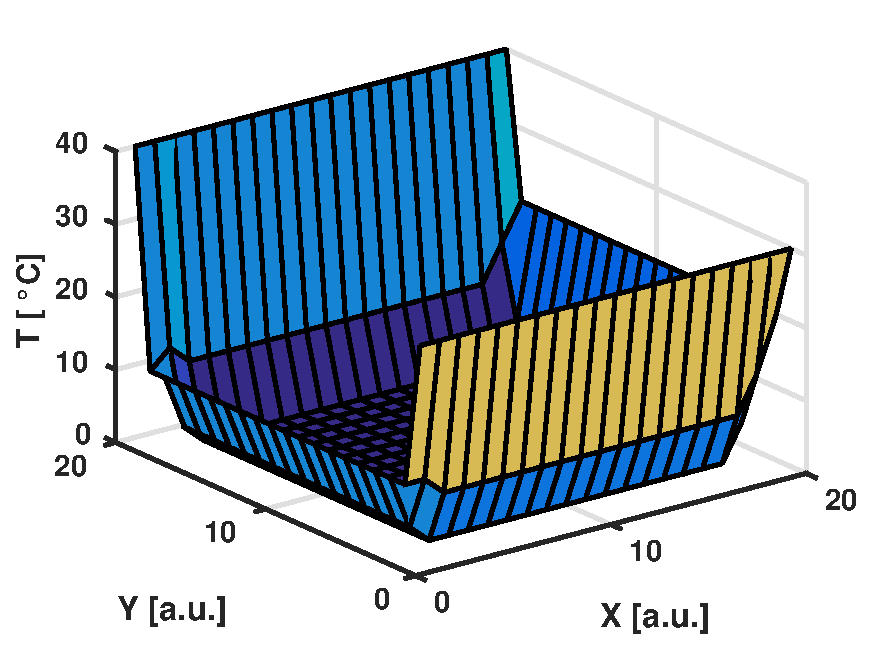
\includegraphics[width=0.5\textwidth]{img/it1}
  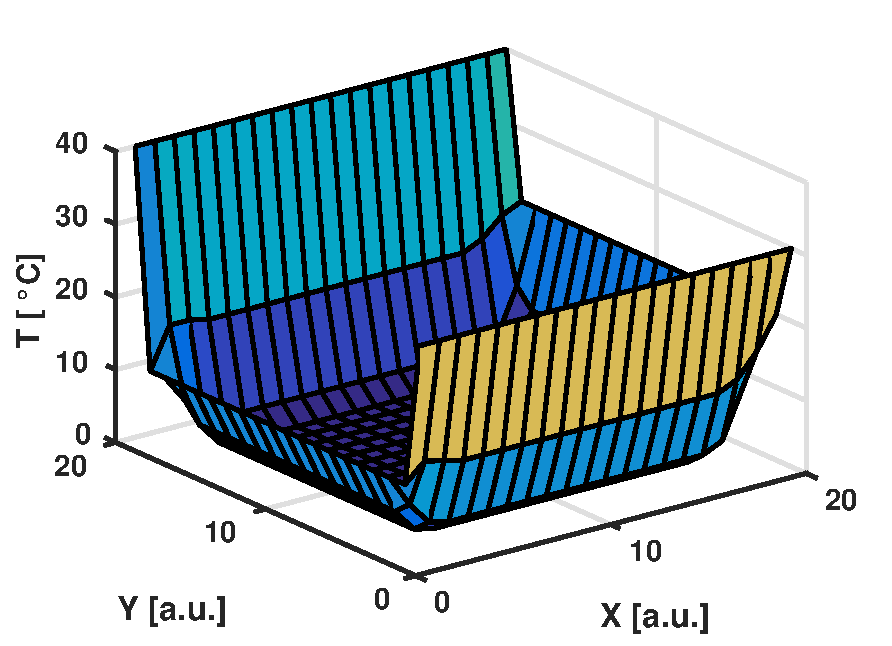
\includegraphics[width=0.5\textwidth]{img/it2}\\
  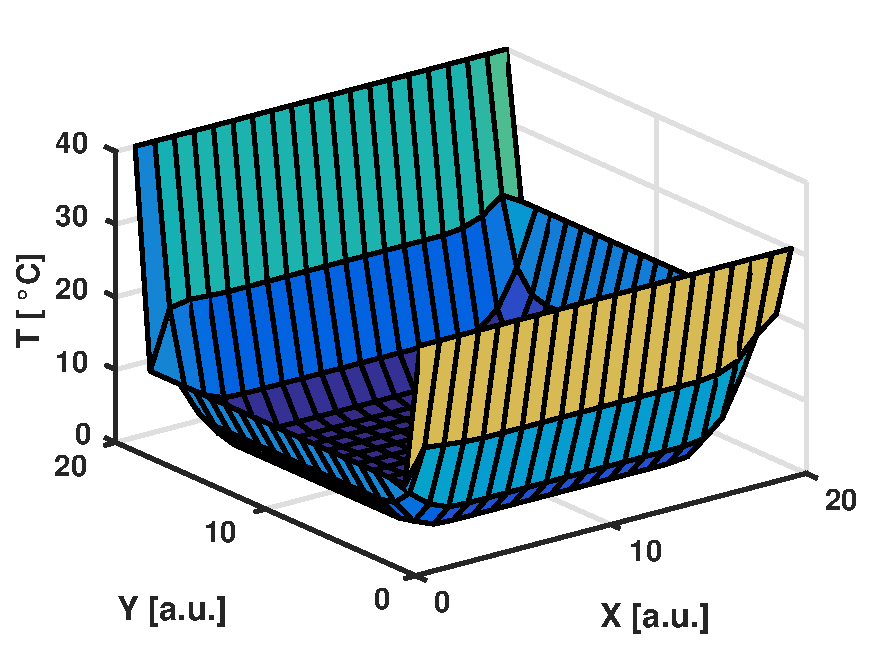
\includegraphics[width=0.5\textwidth]{img/it3}
  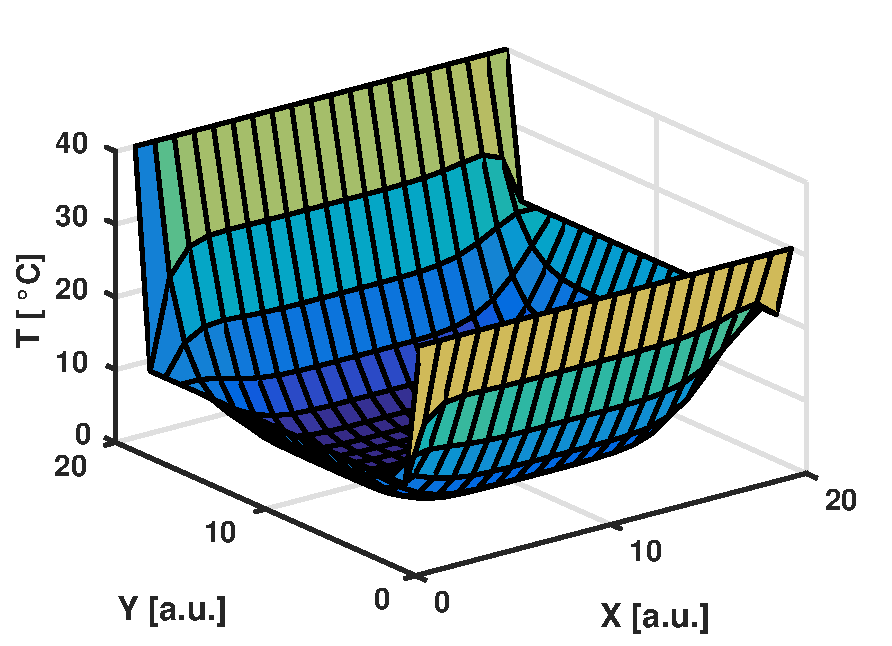
\includegraphics[width=0.5\textwidth]{img/it10}
\end{frame}

\subsection*{Gauss-Seidel method}
\begin{frame}[fragile]
  \frametitle{Gauss-Seidel method}
  The Gauss-Seidel method is quite similar to Jacobi method
  \begin{itemize}
   \item The only difference is that the new estimate $x^\text{new}$ is returned to the solution $x^\text{old}$ as soon as it is completed
   \item For following nodes, the updated solution is used immediately \pause
   \item Our straightforward script (from the Jacobi method) is therefore changed easily:
   \begin{itemize}
    \item Do not create a \lstinline$Tnew$ array (save memory!)
    \item Do not store the solution in \lstinline$Tnew$, but simply in \lstinline$T$
    \item Do not perform the update step \lstinline$T=Tnew$
    \item See \lstinline$laplace_gaussseidel.m$ for the algorithm.\pause
   \end{itemize}
   \item The straightforward script works well for the current Laplace equation, but we define the generic Gauss-Seidel algorithm on the following slides.
  \end{itemize}
\end{frame}

\begin{frame}[fragile]
  \frametitle{Gauss-Seidel method}
  \begin{itemize}
    \item Define a lower and strictly upper triangular matrix, such that $A = L + U$
    \item Now we can solve AT=b by:
    \begin{align*}
      (L+U)T &= b \\
      LT &= b - UT \\
      LT^\text{new} &= b - UT^\text{old} \\
      T^\text{new} &= L^{-1}(b-UT^\text{old})
   \end{align*}
     \item Using the $n$ and $n+1$ notation for old and new time steps, we find in for the general Gauss-Seidel method:
     \[
      x^{n+1} = L^{-1}\left(b-Ux^n\right)
     \]
     \[
      x_i^{n+1} = \frac{1}{A_{ii}}\left(b_i - \sum_{j<i} A_{ij}x_j^{n+1}- \sum_{j>i} A_{ij}x_j^n\right)
     \]
  \end{itemize}
\end{frame}

\section{Summary}
\subsection*{Summary}
\againframe<2>{contents}
\begin{frame}[fragile]
  \frametitle{Summary}
  \begin{itemize}
   \item Partial differential equations can be written as sparse systems of linear equations
   \item Sparse systems can be handled with a direct method like Gaussian elimination
    \item If you have systems of more than 1 dimension, a direct method still can be used, if there are no memory issues, otherwise an iterative method may be attractive.
    \item The Jacobi method was introduced. Many other methods are based on the Jacobi method (SOR method, for example)
  \end{itemize}
\end{frame}
\end{document}
